% --------------------------------------------------------------------
% ----------- CHAPTER 3: SYSTEM DESIGN AND FUNCTIONALITIES -----------
% --------------------------------------------------------------------

% NOTE: Assurez-vous d'avoir ces packages dans votre préambule
% \usepackage{graphicx}
% \usepackage{subcaption}
% \usepackage{tikz}
% \usetikzlibrary{decorations.pathmorphing}
% \usepackage{float} % Essentiel pour le positionnement forcé [H] des figures

\chapter{System Design and Functionalities}
\label{chap:system_design}

The design of a modern tactical diagramming tool for football must reconcile two realities: the increasing availability of spatio-temporal match data, and the continued need for intuitive, expressive manual diagram creation. This chapter presents the complete set of functionalities for such a tool, structured to follow the natural workflow of a coach or analyst. The goal is not merely to list features, but to present a coherent design blueprint where each choice is deliberately justified by established principles in Human-Computer Interaction (HCI), cognitive psychology, and the state of the art in sports analytics \cite{morgulev2018sports, liu2024smartboard, wu2018forvizor, sarmento2014match, munzner2014visualization}.

\vspace{2em}

% --------------------------------------------------------------------
\section{Scenario and Team Initialization}
% --------------------------------------------------------------------

\subsection{Creating \& Analyzing Scenarios}
The first step in any tactical workflow is to establish a context. An effective tool must allow a coach to either analyze a past performance or prepare for a future one. To accommodate this duality, the system is designed to offer two primary entry points:
\begin{itemize}
    \item \textbf{Match-Based Mode ("Tactical View"):} The user can load a complete, processed match. This mode is the foundation for reconstructive analysis, allowing a coach to review key sequences, understand tactical patterns, and prepare sessions grounded in real events. The system is designed to handle datasets containing synchronized player positions and event logs, such as the one provided by the Deutsche Fußball Liga (DFL) \cite{bassek2025integrated}.
    This dataset contain player and ball positions, speed, minute of play and synchronized event tags (passes, shots, fouls, etc...).

    \item \textbf{Empty Pitch Mode ("Strategic View"):} Alternatively, a user can start with a blank canvas. This mode is essential for creative and preparatory tasks: designing drills, establishing a team's default tactical formation, or simulating "what-if" scenarios against a potential opponent.
\end{itemize}
This dual-entry approach is crucial, as coaching workflows frequently alternate between reconstructive analysis and creative planning \cite{sarmento2014match}.

\vspace{1em}

\subsection{Team and Formation Setup}
Once in the "Strategic View," setting up the teams must be a fluid and efficient process.
\begin{itemize}
    \item \textbf{Player Placement and Group Management:} A key design principle is to allow users to drag and drop player tokens directly onto the pitch. To support typical coaching workflows, the system is conceived to allow multi-selection of players, enabling the coach to move entire defensive lines or midfield blocks as a single unit. This aligns with the Gestalt principle of \textbf{Common Region}, where selected items are perceived as a group, simplifying complex manipulations \cite{gestalt}.
    
    \vspace{0.5em}
    
    \item \textbf{Template and Playbook Library:} To accelerate setup, the tool provides a library of common tactical formations (e.g., 4-3-3, 4-4-2). A coach can load a template instantly and then make minor adjustments. Furthermore, any custom formation can be saved back into this library for future reuse. This adheres to Nielsen's fourth heuristic, \textbf{Consistency and Standards}, by providing familiar starting points \cite{nielsen1994heuristics}. The library is also designed to store entire animated plays, creating a "playbook" of set pieces or tactical drills.
    
    \vspace{0.5em}
    
    \item \textbf{Split-Screen Comparison:} A key feature for strategic planning is the ability to compare two tactical setups side-by-side. The split-screen mode allows a coach to display two different formations or variations of a single play simultaneously, facilitating A/B testing of tactical ideas and clarifying instructions for players.
\end{itemize}

\vspace{3em}

% --------------------------------------------------------------------
\section{Core Visualization and Visual Language}
% --------------------------------------------------------------------

The visual foundation of the tool is paramount. Every design choice aims to maximize clarity and minimize the user's cognitive load, ensuring that the interface itself becomes "invisible" so the coach can focus on the tactics \cite{krug2005dontmakeme}.

\vspace{1em}

\subsection{Pitch and Player Representation}
The system renders a proportionally accurate pitch with all standard markings. In the "Tactical View," players are represented as abstract bicolored discs, a deliberate choice over photorealistic avatars.
\begin{itemize}
    \item \textbf{Visual Encoding of Players:} The top half of the disc shows the shirt color, the bottom half the shorts color, and the jersey number is displayed in the center: \hspace{0.5em}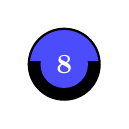
\begin{tikzpicture}[scale=0.45,baseline=-0.6ex]
                \begin{scope}
                    \clip (0,0) circle (1);
                    \fill[black] (-1,-1) rectangle (1,0.1);
                    \fill[blue!70] (-1,0.1) rectangle (1,1);
                \end{scope}
                \fill[blue!70] (0,0) circle (0.67);
                \draw[thick] (0,0) circle (1);
                \node[white] at (0,0) {\textbf{8}};
            \end{tikzpicture}\\
    This abstract representation is effective because it removes extraneous visual details, allowing the coach and players to focus solely on positioning and structure. This is a direct application of Tufte's principle of maximizing the "data-ink ratio" by removing non-essential visual elements \cite{tufte1991envisioning}.
    
    \vspace{0.5em}
    
    \item \textbf{Orientation and Speed Indicator:} A small arrow is attached to each player token. Its direction indicates the player's orientation (calculated from smoothed trajectory vectors), and its length is directly proportional to their speed. This design is scientifically grounded in the theory of \textbf{pre-attentive visual processing} \cite{ware2013information}. The human brain can decode variations in length and orientation almost instantly, without conscious effort. Displaying speed as a number (e.g., "25 km/h") would require the user to read and process each number individually, drastically increasing cognitive load and cluttering the interface. The player's number and the attached arrow rotate in unison with the player's real orientation, providing an immediate and intuitive visual cue of where the player is looking and moving.

    \item \textbf{Why orientation matters:} In tactical analysis, a player's body orientation is one of the most critical variables for interpreting marking, pressing, and passing options. The direction a player is facing influences their effective field of view, available passing lanes, and reaction time to pressing triggers. Encoding this visually through an arrow is significantly more efficient than relying on numerical metrics or textual labels: orientation can be decoded in less than 200 milliseconds via pre-attentive visual processing, whereas reading values takes conscious effort and interrupts tactical reasoning.

\end{itemize}

\vspace{1em}

\subsection{A Proposed Visual Language for Tactical Actions}
To address the lack of standardization in football diagrams noted in the literature \cite{walsh2023lack}, a central goal of this design is to propose a consistent visual language. This language distinguishes between the data-driven "Tactical View" and the more abstract "Strategic View."
\begin{itemize}
    \item \textbf{Player States in "Strategic View":} For purely hypothetical scenarios, a simplified representation is proposed to clearly distinguish roles:
        \begin{itemize}
            \item 
\begin{tikzpicture}[scale=0.45,baseline=-0.6ex] \draw[red, thick] (0,0) circle (0.7); \end{tikzpicture} \quad Attacker (non-ball carrier)
            \vspace{0.5em}
            \item 
\begin{tikzpicture}[scale=0.45,baseline=-0.6ex] \draw[very thick, red] (0,0) circle (0.8); \draw[red, thick] (0,0) circle (0.6); \end{tikzpicture} \quad Ball carrier
            \vspace{0.5em}
            \item 
\begin{tikzpicture}[scale=0.5,baseline=-0.6ex] \node[blue, thick] at (0,0) {\Huge $\times$}; \end{tikzpicture} \quad Defender
        \end{itemize}
        
        \vspace{1em}
        
    \item \textbf{Arrow Types:} Different arrow styles correspond to specific actions, creating a clear visual grammar across all modes:
        \begin{itemize}
            \item 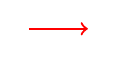
\begin{tikzpicture}[scale=0.5,baseline=-0.6ex] \draw[->, thick, red] (0,0) -- (1.5,0); \end{tikzpicture} \quad Pass
            \vspace{0.5em}
            \item 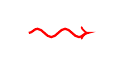
\begin{tikzpicture}[scale=0.5,baseline=-0.6ex] \draw[->, thick, red, decorate, decoration={snake, amplitude=1.5}] (0,0) -- (1.5,0); \end{tikzpicture} \quad Dribble
            \vspace{0.5em}
            \item \begin{tikzpicture}[scale=0.5,baseline=-0.6ex] \draw[->, thick, red, dashed] (0,0) -- (1.5,0); \end{tikzpicture} \quad Attacking Off-ball run
            \vspace{0.5em}
            \item \begin{tikzpicture}[scale=0.5,baseline=-0.6ex] \draw[->, thick, blue, dashed] (0,0) -- (1.5,0); \end{tikzpicture} \quad Defensive run / Pressing
        \end{itemize}
\end{itemize}

\vspace{1em}

\subsection{Data-Driven Analytical Overlays}
To move beyond simple description, an effective tool must help the coach to see the game's hidden dynamics. The system is therefore designed to superimpose data-driven analytical layers onto the pitch.

\vspace{1em}

\textbf{Pressure Visualization:} The tool can visualize the defensive pressure experienced by the ball carrier. This is represented visually as a dynamic "aura" around the player. Its color and intensity change based on a real-time calculation of the proximity, speed, and angle of nearby defenders, using models inspired by recent academic work \cite{bekkers2024pressing}. This provides an immediate, intuitive understanding of the player's available options and the stress they are under, translating complex data into a simple visual heuristic.

\vspace{0.5em}

\textbf{Why an aura is more effective than numbers:} Defensive pressure is a dynamic, rapidly changing variable. Displaying it as a real-time numeric value forces the analyst to read, interpret, and mentally map it to the spatial situation — a slow, cognitively costly process. By contrast, a colored aura directly leverages the visual system's ability to process gradients and intensities instantly, making it possible to “feel” the pressure level at a glance. This mirrors the way players themselves perceive pressure on the pitch: not as a number, but as a spatial sense of opponents closing in.

\vspace{0.5em}
    
\textbf{Contextual Tactical Zones:} For advanced analysis, the tool is designed to render real-time tactical zones that reveal hidden opportunities and risks. These overlays transform the tool from a descriptive platform ("what happened") to a prescriptive one ("what could happen"), actively guiding the coach's tactical decision-making.
        \begin{itemize}
            \item \textbf{Passing Channels:} Blocked passing options are visualized as flexible ellipses based on opponent positioning, similar to concepts of "pitch control" explored in `PassVizor` \cite{xie2020passvizor}. The visualization uses a clear color code:
            \begin{itemize}
                \item 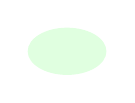
\begin{tikzpicture}[scale=0.5,baseline=-0.6ex] \fill[green!30, opacity=0.4] (0,0) ellipse (1 and 0.6); \end{tikzpicture} \quad Safe channels
                \item 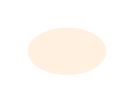
\begin{tikzpicture}[scale=0.5,baseline=-0.6ex] \fill[orange!30, opacity=0.4] (0,0) ellipse (1 and 0.6); \end{tikzpicture} \quad Risky channels
                \item 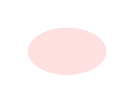
\begin{tikzpicture}[scale=0.5,baseline=-0.6ex] \fill[red!30, opacity=0.4] (0,0) ellipse (1 and 0.6); \end{tikzpicture} \quad Impossible/Blocked channels
            \end{itemize}
            
            \vspace{0.5em}
            
            \item \textbf{Shooting Zones:} 
\begin{tikzpicture}[scale=0.5,baseline=-0.6ex]
                \fill[green!40, opacity=0.4] (0,-0.5) -- (-1,1) -- (-0.33,1) -- cycle;
                \fill[orange!40, opacity=0.4] (0,-0.5) -- (-0.33,1) -- (0.33,1) -- cycle;
                \fill[red!40, opacity=0.4] (0,-0.5) -- (0.33,1) -- (1,1) -- cycle;
                \end{tikzpicture} A cone projected from the player indicates the areas with the highest probability of scoring. The cone's gradient from green (high probability) to red (low probability) is envisioned to be calculated in real time based on the player's distance to goal, shooting angle, and the positioning of the goalkeeper and nearby defenders. This design is inspired by spatial shot effectiveness patterns identified in academic analyses such as \cite{perez2025shooting}, which highlight how these variables influence scoring likelihood in match situations.
        \end{itemize}


\vspace{3em}

% --------------------------------------------------------------------
\section{Temporal Navigation and View Management}
% --------------------------------------------------------------------
\subsection{The Timeline System}
The timeline is the central hub for temporal control, designed for both high-level Browse and micro-analysis. It provides a powerful workflow for navigating to key moments, as illustrated in the figures that follow.

\begin{itemize}
    \item \textbf{Slider and Event Markers:} The main slider allows for fluid, frame-by-frame scrubbing through the match. Initially, key match events are all displayed as clickable icons on the timeline. This design respects \textbf{Jakob's Law}, as users are already familiar with this interaction pattern from standard video editing software, reducing the learning curve \cite{jakobslaw}.

    \vspace{0.5em}

    \item \textbf{Event Filtering:} In a typical match, the sheer number of events can lead to a cluttered and overwhelming timeline. To address this, the tool provides an event filter panel. A user can select specific event types (e.g., "Goal"), and the timeline instantly updates to show only those relevant markers. This is a direct application of \textbf{Hick's Law}; by drastically reducing the number of choices presented to the user, the system makes it significantly faster and easier to find important moments, thus reducing cognitive strain \cite{hickslaw}.

    \vspace{0.5em}

    \item \textbf{Direct Navigation and Micro-Zoom:} Clicking on a specific event marker on the timeline serves two functions simultaneously. First, it instantly navigates the main view to that precise frame in the match. Second, it displays a zoomed-in, secondary timeline focused on the moments immediately preceding and following the selected event. This micro-navigation view is crucial for detailed analysis of the build-up and consequences of a key action, providing context without requiring the user to manually scrub back and forth.
\end{itemize}

\begin{figure}[H]
    \centering
    \includegraphics[width=0.9\textwidth]{Figures/FILTERING.png}
    \caption{\textbf{Step 1 - Filtering :} Filtering what type of events we want to have above the timeline.}
    \label{fig:timeline_unfiltered}
\end{figure}

\begin{figure}[H]
    \centering
    \includegraphics[width=0.9\textwidth]{Figures/PRE_SELECTION.png}
    \caption{\textbf{Step 2 - Pre-selection :} Events are filtered and now the user chooses what action to select.}
    \label{fig:timeline_filtered}
\end{figure}

\begin{figure}[H]
    \centering
    \includegraphics[width=0.9\textwidth]{Figures/SELECTION.png}
    \caption{\textbf{Step 3 - Selection :} When clicking on a specific event (here, "Blue team scores"), we zoom in so that the user can better see the other events around this goal. After clicking we are projected at the goal moment.}
    \label{fig:timeline_action_zoom}
\end{figure}

\vspace{1em}

\subsection{Camera Management}
The camera system is designed to focus attention effectively, providing a flexible viewport onto the tactical canvas. A dedicated control panel offers a suite of ten specialized buttons, each addressing a specific analytical need. The panel is organized into three logical groups: manual controls, automated views, and presets for key zones.

\begin{itemize}
    \item \textbf{Manual Controls:} The default view shows the entire pitch. The user has direct control via three essential buttons: standard `+` and `-` buttons allow for manual zoom, while a `Reset` button instantly restores the full-pitch view. These controls are designed to be large and immediately accessible, respecting \textbf{Fitts' Law} to minimize interaction time and effort \cite{fittslaw}.
    
    \vspace{0.5em}
    
    \item \textbf{Automated and Intelligent Views:} To reduce the manual burden on the user, two intelligent modes are provided:
        \begin{itemize}
            \item \textbf{Ball Tracking (`BALL`):} A dedicated mode that automatically centers the camera on the ball and follows its movement, freeing the coach to focus on the tactical context rather than manual navigation.
            \item \textbf{Context-Aware Auto-Zoom:} The tool is designed with an intelligent camera that adapts to the play. It can automatically zoom in on the ball carrier during close control and then zoom out to a wider view when a long pass is anticipated. This reduces the need for constant manual adjustment, lowering the user's extraneous cognitive load.
        \end{itemize}
        
    \vspace{0.5em}
    
    \item \textbf{Preset Views for Set Pieces and Key Zones:} To accelerate the analysis of recurring situations, the system includes six preset camera views that instantly focus on critical areas of the pitch:
        \begin{itemize}
            \item \textbf{Corners (`TLC`, `TRC`, `BLC`, `BRC`):} These four buttons instantly focus the camera on the top-left, top-right, bottom-left, and bottom-right corners, essential for detailed analysis of offensive and defensive corner-kick organizations.
            \item \textbf{Penalty Areas (`LP`, `RP`):} These two buttons zoom in on the left and right penalty areas, crucial for analyzing dangerous attacking situations, finishing, or defensive organization in the final third.
        \end{itemize}
    This set of dedicated presets acts as a series of "accelerators" in the sense of Nielsen's heuristics, allowing expert users to navigate to critical zones with a single click instead of multiple zoom and pan operations \cite{nielsen1994heuristics}.
\end{itemize}

\vspace{3em}
% --------------------------------------------------------------------
\section{Tactical Annotation and Simulation}
% --------------------------------------------------------------------

A central component of the tool is its ability to translate tactical ideas into clear, structured visual annotations. This functionality serves two purposes: it enables coaches to convey concepts rapidly to players, and it provides a visual record that can be revisited, adjusted, and compared over time.

\subsection{Annotation Tools}

The annotation system is deliberately designed to be both expressive and precise. It offers a range of tools that balance the creative freedom needed for tactical ideation with the clarity required for effective communication.

\textbf{Cognitive efficiency of visual annotations:} Each annotation type (arrow, zone, label) is designed to carry meaning through shape, style, and position without requiring the viewer to consult a legend constantly. This reduces working memory load and speeds up comprehension during live or fast-paced tactical reviews.


\begin{itemize}
    \item \textbf{Arrow Creation and Properties:} Beyond simply drawing arrows, the user can customize a comprehensive set of properties:
    \begin{itemize}
        \item \textit{Color and Style:} Passes, dribbles, and runs follow the visual grammar established earlier (solid, dashed, wavy lines), but users can override these defaults to emphasize specific tactical ideas. Color selection is offered via a perceptually uniform palette to ensure high contrast and accessibility, particularly in projected presentations.
        \item \textit{Thickness and Curvature:} Line thickness can encode the importance or intensity of an action (e.g., a high-speed pass rendered thicker). Curvature can be adjusted to reflect realistic ball trajectories or to depict off-ball runs that bend around defenders.
        \item \textit{Arrowheads and Endpoints:} Multiple arrowhead styles are available (classic, triangular, open), enabling coaches to visually distinguish between action types or player intentions.
    \end{itemize}

    These properties are not merely aesthetic: they serve as cognitive cues, allowing players to interpret a diagram faster and with less ambiguity. By encoding action type, importance, and trajectory directly into the shape and style of an arrow, the tool exploits \textbf{pre-attentive visual attributes} \cite{ware2013information}, reducing the need for explanatory text.

    \vspace{0.5em}

    \item \textbf{Zone Creation and Properties:} Zones can be drawn as rectangles, circles, ellipses, or free-form polygons. Each zone supports:
    \begin{itemize}
        \item Fill color and opacity (to avoid obscuring underlying data).
        \item Border style and thickness.
        \item Optional labels for naming tactical areas (e.g., ``pressing trap zone'', ``shooting pocket'').
    \end{itemize}
    This flexibility supports both schematic training diagrams and precise, data-driven overlays.

    \vspace{0.5em}

    \item \textbf{Post-Creation Editing:} All annotations are fully editable after creation. Users can drag endpoints, rotate arrows, adjust curvature, or recolor elements in real-time. A live preview ensures that changes are immediately visible.

    \vspace{0.5em}

    \item \textbf{Advanced Interaction Features:} To support complex tactical drawings:
    \begin{itemize}
        \item \textit{Multi-Selection \& Grouping:} Multiple annotations can be selected and moved or modified together, useful when adjusting an entire defensive line or a coordinated pressing pattern.
        \item \textit{Layer Management:} Annotations are organized into layers, which can be shown or hidden. This allows, for example, a coach to toggle between offensive and defensive phases without redrawing.
        \item \textit{Annotation Presets:} Frequently used styles (e.g., a standard ``pressing arrow'') can be saved as presets for rapid reuse, accelerating workflow in live sessions.
        \item \textit{Layer Visibility Toggles:} Each annotation layer (e.g., \texttt{Offense Layer}, \texttt{Defense Layer}, \texttt{Set Pieces Layer}) can be individually toggled on or off via a dedicated “eye” icon in the \texttt{Layers Panel}. This allows the coach to instantly switch between viewing only offensive annotations, only defensive ones, or any desired combination. The visibility state is updated in real time without reloading the scene. This selective display is particularly valuable when illustrating different phases of play: hiding non-relevant layers keeps the visual scene clean and prevents cognitive overload, avoiding the “visual noise” problem that occurs when all tactical information is displayed simultaneously.

    \end{itemize}

    \vspace{0.5em}

    \item \textbf{Undo/Redo \& Cognitive Safety Nets:} A robust undo/redo system encourages exploration by removing the fear of making irreversible mistakes, aligning with the principle of \textbf{User Control and Freedom} \cite{nielsen1994heuristics}.

    \item \textbf{Grouped Deletion Tools:} Instead of relying solely on “Clear All,” the tool supports deletion by annotation group. In the \texttt{Layers Panel}, a coach can select an entire layer (e.g., all pressing arrows, or all set-piece zones) and remove it with a single click. This prevents accidental loss of unrelated work and allows for fast iteration during tactical discussions: an entire scenario can be reworked without having to manually erase each element.

\end{itemize}

\vspace{1em}

\subsection{Simulation Mode}
\label{sec:sim_mode_design}

The simulation mode extends the tool beyond static diagrams, enabling dynamic ``what-if'' analyses. Its design choices reflect the need to experiment with tactical variations without overwhelming the user.

\begin{itemize}
    \item \textbf{Loop-Based Scenario Editing:} A coach selects a time interval (e.g., five seconds before a goal), which then plays in a continuous loop. This fixed temporal context supports repeated observation and modification without constant manual navigation.

    \item \textbf{From Annotation to Action:} In simulation mode, attaching an arrow to a player overrides their recorded trajectory. The player then moves according to the drawn instruction, and the resulting new play unfolds on screen. This \textbf{direct manipulation} approach \cite{shneiderman1983direct} creates an immediate cause-effect link between coach input and visual output, strengthening tactical understanding.

    \item \textbf{Proportional Timing:} The time taken to execute a simulated action scales with the length of the drawn arrow, providing an intuitive, non-verbal way to encode tempo and intensity.

    \item \textbf{Trajectory Fading for Clarity:} Both real and simulated trajectories gradually fade as the play progresses, instead of remaining fully visible. This is a deliberate decision grounded in cognitive load theory: displaying all past paths simultaneously produces excessive visual clutter (often called ``spaghetti diagrams'' in sports analytics). The fading preserves short-term context—so the user can still see the immediate origin of a movement—while keeping the scene readable. This design follows Tufte's principle of reducing non-essential ``data-ink'' \cite{tufte1991envisioning}  and reduces cognitive load by emphasizing the latest movements.
    
    \item \textbf{Branching Scenarios:} The system supports multiple alternative simulations from the same starting point. A coach can compare Variant A (e.g., pass to left wing) against Variant B (pass into the box) without overwriting the original data.

    \item \textbf{Trigger Points:} Simulated actions can be set to trigger only when specific conditions are met (e.g., a forward run begins only once a midfielder enters a certain zone), allowing for more realistic tactical modeling.

    \item \textbf{Export and Communication:} Simulations can be recorded and exported as short video clips, facilitating clear communication to players or inclusion in scouting reports.
\end{itemize}

\paragraph{Action model driven by annotations (common to Tactical \& Strategic views).}
Beyond simple motion overrides, the simulation treats an annotated arrow as a typed action that binds one or two players to a football event (e.g., \emph{pass}, \emph{shot}, \emph{dribble}, \emph{tackle}). In Tactical View (match data), the user may slightly reposition players and draw a typed arrow; this produces a \emph{user-authored action} that (i) overrides trajectories locally for playback and (ii) prepares an updated event entry aligned to the edited frames. In Strategic View (blank pitch), the same authoring pattern creates hypothetical actions with the exact same schema. This unified interaction keeps the mental model identical across views: draw $\rightarrow$ bind player(s) $\rightarrow$ choose action type $\rightarrow$ simulate.


In designing the simulation system, the guiding principle has been to make complex tactical ideas \textbf{fast to draw, easy to read, and faithful to the intended meaning}, while minimizing the risk of misinterpretation. The trajectory fading mechanism, in particular, illustrates how a small visual design choice can have a large impact on the usability of a sports analysis tool.


% --------------------------------------------------------------------
\section{Customization and Project Management}
% --------------------------------------------------------------------

Finally, the tool provides options for personalization and saving work.

\subsection{Interface Customization}
A well-designed tactical tool must be visually clear in a variety of contexts, from a high-resolution monitor in an analyst's office to a low-quality projector in a team meeting room. To address this, the tool's design incorporates a robust system for interface customization, centered on perceptually effective visual themes.

\begin{figure}[H]
    \centering
    \begin{subfigure}[b]{0.48\textwidth}
        \centering
        \includegraphics[width=\textwidth]{Figures/THEME-CLASSIC.png}
        \caption{The "Classic" visual theme.}
        \label{fig:theme_classic}
    \end{subfigure}
    \hfill
    \begin{subfigure}[b]{0.48\textwidth}
        \centering
        \includegraphics[width=\textwidth]{Figures/THEME-BLACK-AND-WHITE.png}
        \caption{The "Black \& White" theme.}
        \label{fig:theme_bw}
    \end{subfigure}
    \caption{The two primary visual themes available in the application.}
    \label{fig:themes}
\end{figure}


As introduced earlier with the orientation arrows, our colour choices are optimised only for certain visual overlays rather than for the entire scene.
In practice, this means focusing on the offside line and player-orientation arrows, while keeping the pitch, pitch lines, and team kits fixed to match the real match or training context.
The reason is simple: these overlays carry critical analytical information and must remain easy to read regardless of the colours on the pitch.
If, for example, the offside line or arrows were too close in colour to the grass or a team’s kit, they would blend into the background and lose their function.
By optimising only overlays, we target the elements where colour choice has the greatest impact on tactical clarity, without altering the recognisable appearance of the game.

\begin{itemize}
    \item \textbf{Visual Themes:} As shown in Figure \ref{fig:themes}, the design includes two primary themes. The rationale for this is not merely aesthetic. Professional team kits often feature colors that have poor contrast against each other or against the green of the pitch, which can make player identification difficult. This is a critical issue for coaches who need immediate clarity, and especially for users with color vision deficiencies. 
    
    To solve this, the themes are generated by an algorithm whose goal is to maximize legibility. The system is designed to operate in a \textbf{perceptually uniform color space}, which models human color vision far more accurately than standard screen-based color models like RGB \cite{ware2013information}. By optimizing for the highest possible perceived difference between colors, the themes guarantee strong contrast and accessibility.
    
    \vspace{0.5em}
    
    \item \textbf{User Control:} While the system provides an algorithmically optimized default, the principle of \textbf{User Control and Freedom} is paramount \cite{nielsen1994heuristics}. The user retains final control and can manually override the theme's colors or change the global scale of all visual elements on the pitch via a dedicated settings panel. This allows for adaptation to personal preferences, specific presentation needs, or unexpected lighting conditions.
\end{itemize}

\vspace{1em}

\subsection{Saving and Exporting}
\begin{itemize}
    \item \textbf{Saving and Loading:} The system allows for saving the full project state, including loaded data, all annotations, camera positions, and filter settings. In "Strategic Mode," coaches can also save specific team line-ups as reusable templates.
    \item \textbf{Exporting (Envisioned):} For communication, the ability to export is crucial. The tool is envisioned to export annotated frames as static images (PNG, PDF) and animated sequences as videos (MP4), a need consistently highlighted in surveys of professional coaching workflows \cite{lolli2025data}.
\end{itemize}